%%%%%%%%%%%%%%%%%%%%%%%%%%%%%%%%%%%%%%%%%
% Short Sectioned Assignment
% LaTeX Template
% Version 1.0 (5/5/12)
%
% This template has been downloaded from:
% http://www.LaTeXTemplates.com
%
% Original author:
% Frits Wenneker (http://www.howtotex.com)
%
% License:
% CC BY-NC-SA 3.0 (http://creativecommons.org/licenses/by-nc-sa/3.0/)
%
%%%%%%%%%%%%%%%%%%%%%%%%%%%%%%%%%%%%%%%%%

%----------------------------------------------------------------------------------------
%	PACKAGES AND OTHER DOCUMENT CONFIGURATIONS
%----------------------------------------------------------------------------------------

\documentclass[paper=a4, fontsize=11pt]{scrartcl} % A4 paper and 11pt font size

\usepackage[T1]{fontenc} % Use 8-bit encoding that has 256 glyphs
\usepackage{fourier} % Use the Adobe Utopia font for the document - comment this line to return to the LaTeX default
\usepackage[english]{babel} % English language/hyphenation
\usepackage{amsmath,amsfonts,amsthm} % Math packages
\usepackage{graphicx} % figures
\usepackage{listings} % Required for insertion of code

\usepackage{lipsum} % Used for inserting dummy 'Lorem ipsum' text into the template

\usepackage{sectsty} % Allows customizing section commands
\allsectionsfont{\centering \normalfont\scshape} % Make all sections centered, the default font and small caps

\usepackage{fancyhdr} % Custom headers and footers
\pagestyle{fancyplain} % Makes all pages in the document conform to the custom headers and footers
\fancyhead{} % No page header - if you want one, create it in the same way as the footers below
\fancyfoot[L]{} % Empty left footer
\fancyfoot[C]{} % Empty center footer
\fancyfoot[R]{\thepage} % Page numbering for right footer
\renewcommand{\headrulewidth}{0pt} % Remove header underlines
\renewcommand{\footrulewidth}{0pt} % Remove footer underlines
\setlength{\headheight}{13.6pt} % Customize the height of the header

\numberwithin{equation}{section} % Number equations within sections (i.e. 1.1, 1.2, 2.1, 2.2 instead of 1, 2, 3, 4)
\numberwithin{figure}{section} % Number figures within sections (i.e. 1.1, 1.2, 2.1, 2.2 instead of 1, 2, 3, 4)
\numberwithin{table}{section} % Number tables within sections (i.e. 1.1, 1.2, 2.1, 2.2 instead of 1, 2, 3, 4)

\setlength\parindent{0pt} % Removes all indentation from paragraphs - comment this line for an assignment with lots of text

\lstset{
   extendedchars=true,
   basicstyle=\footnotesize\ttfamily,
   showstringspaces=false,
   showspaces=false,
   numbers=left,
   numberstyle=\footnotesize,
   numbersep=10pt,
   tabsize=4,
   breaklines=true,
   showtabs=false,
   captionpos=b
}

%----------------------------------------------------------------------------------------
%	TITLE SECTION
%----------------------------------------------------------------------------------------

\newcommand{\horrule}[1]{\rule{\linewidth}{#1}} % Create horizontal rule command with 1 argument of height

\title{	
\normalfont \normalsize 
\textsc{Udacity Data Analyst Nanodegree} \\ [25pt] % Your university, school and/or department name(s) % OVERRIDE
\horrule{0.5pt} \\[0.4cm] % Thin top horizontal rule
\LARGE{Project 1} \\ % The assignment title % SIZE OVERRIDE
\horrule{0.5pt} \\[0.5cm] % Thick bottom horizontal rule
}

\author{Ming Wen} % Your name % OVERRIDE

\date{\normalsize\today} % Today's date or a custom date

\begin{document}

\maketitle % Print the title

%----------------------------------------------------------------------------------------
%	PROBLEM 1
%----------------------------------------------------------------------------------------

\section{Test a Perceptual Phenomenon}

\subsection{Idenfity variables in the experiment}
\medskip
\noindent\fbox{
	\parbox{\textwidth}{
        What is our independent variable?
        What is our dependent variable?
	}
}
\medskip

In this experiment, the independent variable is congruence or
incongruence of words and colors. The dependent variable is
the time of response under each condition.

\subsection{Establish a hypothesis and statistical test}
\medskip
\noindent\fbox{
	\parbox{\textwidth}{
        What is an appropriate set of hypotheses for this task?
        What kind of statistical test do you expect to perform?
        Justify your choices.
	}
}
\medskip

The null hypothesis $H_0$: for the whole population,
the mean time of response under congruent
condition is greater than or equal to the mean time of response under
incongruent condition.

The alternative hypothesis $H_A$: for the whole population,
the mean time of response under congruent
condition is less than the mean time of response
under incongruent condition.

Since we don't have information about the population mean, the t-test
should be used. From common sense we believe that time under
incongruent condition should be greater than time under
congruent condition, so a one-tail test is setup.
And finally, this test is classified as dependent samples t-test
because each participant appears in both groups.

\subsection{Report descriptive statistics}
\medskip
\noindent\fbox{
	\parbox{\textwidth}{
        Report some descriptive statistics regarding this dataset.
        Include at least one measure of central tendency and
        at least one measure of variability.
	}
}
\medskip

Here we define some notations of statistics.

\begin{itemize}
    \item $\bar{t}_c$: the mean time under congruent condition
    \item $\bar{t}_i$: the mean time under incongruent condition
    \item $\bar{t}_d$: the mean of time difference
        (congruence - incongruence)
    \item $s_c$: the sample standard deviation of time under
        congruent condition
    \item $s_i$: the sample standard deviation of time under
        incongruent condition
    \item $s_d$: the sample standard deviation of time difference
    \item $n$: the sample size (of either condition)
\end{itemize}

The sample size of each group is 24.

The mean time under congruent condition $\bar{t}_c = 14.05$.
Its sample standard deviation is $s_c = 3.56$.

The mean time under incongruent condition $\bar{t}_i = 22.02$.
Its sample standard deviation is $s_i = 4.80$.

\subsection{Plot the data}
\medskip
\noindent\fbox{
	\parbox{\textwidth}{
        Provide one or two visualizations that show the distribution
        of the sample data. Write one or two sentences noting what you
        observe about the plot or plots.
	}
}
\medskip

\clearpage
\begin{figure}[h!]
    \centering
    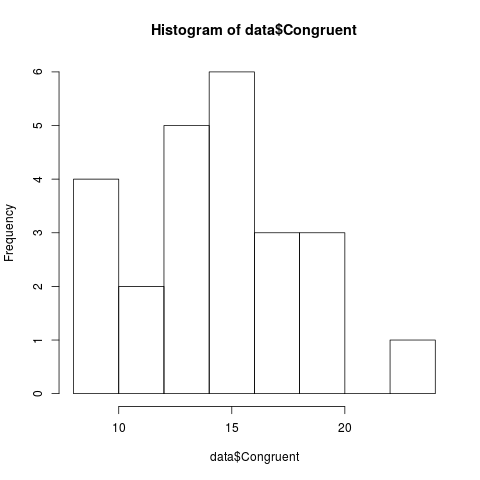
\includegraphics[width=0.6\textwidth]{hist_congruent.png}
    \caption{Histogram of Congruent Condition.}
    \label{fig:hist-congruent}
\end{figure}

\begin{figure}[h!]
    \centering
    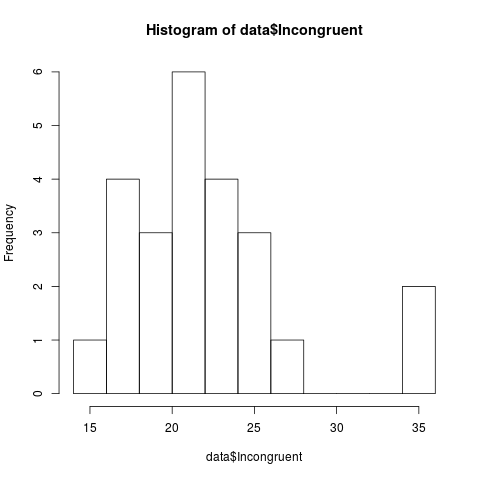
\includegraphics[width=0.6\textwidth]{hist_incongruent.png}
    \caption{Histogram of Incongruent Condition.}
    \label{fig:hist-incongruent}
\end{figure}

The two plots have are similar in these aspects:
\begin{itemize}
    \item Looks like normal distribution. The frequency in the middle
        is greater than each tail.
    \item Outliers exist at the right tail.
\end{itemize}

However, the mean in the second plot is greater than the first, and
its variance is also larger.

\subsection{Perform the statistical test and interpret your results}
\medskip
\noindent\fbox{
	\parbox{\textwidth}{
        What is your confidence level and your critical statistic
        value? Do you reject the null hypothesis or fail to reject it?
        Come to a conclusion in terms of the experiment task.
        Did the results match up with your expectations?
	}
}
\medskip

The difference of means between two groups
is $\bar{t}_d = \bar{t}_c-\bar{t}_i = -7.96$.

The standard error is given by
\begin{equation}
    SE = \frac{s_d}{\sqrt{n}} = \frac{4.86}{4.90} = 0.99.
\end{equation}

Thus the t-value is
\begin{equation}
    t = \frac{\bar{t}_d}{SE} = \frac{-7.96}{0.99} = -8.02.
\end{equation}

If the significant level $\alpha = 0.05$, since the degree of
freedom is $df = 24-1 = 23$, the one-tail t critical value is
$t_{critical} = -1.71$, and the two-tail t critical value should be 
$t_{critical2} = \pm 2.07$.

The confident interval is 
\begin{equation}
    (\bar{t}_d - t_{critical2} * SE,
    \bar{t}_d + t_{critical2} * SE)
    \ = \ (-10.01, \; -5.91)
\end{equation}

Since $t < t_{critical}$, we reject the null hypothesis and
favor the alternative hypothesis.
So in the population, the mean time of response under
congruent condition is less than
that under incongruent condition.

Also from this experiment, we have 95\% of confidence that in the
population, the mean time of response under congruent condition is
$10.01 \; sec$ to $5.91 \; sec$ less than the mean time
of response under incongruent condition.

Those results do conform to our expectations.

\end{document}

